\documentclass[a4paper]{article}

\usepackage{amsmath}
\usepackage{amsfonts}
\usepackage{anysize}
\usepackage{enumerate}
\usepackage{float}
\usepackage{graphicx}
\usepackage{hyperref}
\usepackage{listings}
\usepackage{SIunits}

\marginsize{2.5cm}{2.5cm}{1.5cm}{1.5cm}
\setlength{\parindent}{0pt}

\graphicspath{{./images/}}

\lstset{
    language=vhdl,
    numbers=left,
    xleftmargin=4em
}

\title{Design of Digital Platforms}
\author{Pieter Maene}
\date{\today}

\begin{document}

\maketitle

\section{Analysis of Winter Design}

The design we built for the winter evaluation had the performance metrics listed in Table~\ref{tab:performance_metrics_winter} and the synthesis results from Table~\ref{tab:synthesis_results_winter}. Four shared memory locations (for the parameters, the modulus and the result) were used to communicate between the microprocessor and the coprocessor. Three ports ($P0$, $P1$ and $P3$) were used to send instructions and status information. The exponentiation was fully implemented in hardware, with the software sending instructions to initialise the different parameters and start the exponentiation.\\

\begin{table}[H]
	\begin{center}	
		\begin{tabular}{l|r|r}
			 & \textbf{Encryption} & \textbf{Decryption}\\\hline
			\textbf{Registers} (Bit) & 12351 & 12351\\
		 	\textbf{Clock Cycles} & 69456 & 3073095\\
		\end{tabular}
	\end{center}
	\caption{Performance Metrics---Winter}
	\label{tab:performance_metrics_winter}
\end{table}

\begin{table}[H]
	\begin{center}	
		\begin{tabular}{c|c}
			\textbf{Slices} & 16153 (63\%)\\
			\textbf{Slice FFs} & 12370 (24\%)\\
			\textbf{4 Input LUTs} & 30723 (60\%)\\
			\textbf{Maximum Frequency} & 11.679 \mega\hertz
		\end{tabular}
	\end{center}
	\caption{Synthesis Results --- Winter}
	\label{tab:synthesis_results_winter}
\end{table}

Analysing this data, we can see the design had some serious drawbacks. First, the design was simply too large. It used 63\% of the available slices on the selected FPGA and needed 12 large registers. This resulted from the fact that we used several data paths (one for the decoder, a second for the exponentiation and a third for the Montgomery multiplication), each with its own registers, instead of integrating them. Secondly, because we didn't optimise the critical path, the clock frequency was limited to 11.679 \mega\hertz. This meant that despite the relatively low number of clock cycles, the execution time was not optimal. Finally, implementing the exponentiation algorithm completely in hardwire made optimisations (and particularly algorithmic optimisations) a lot harder.

\begin{figure}[H]
	\center{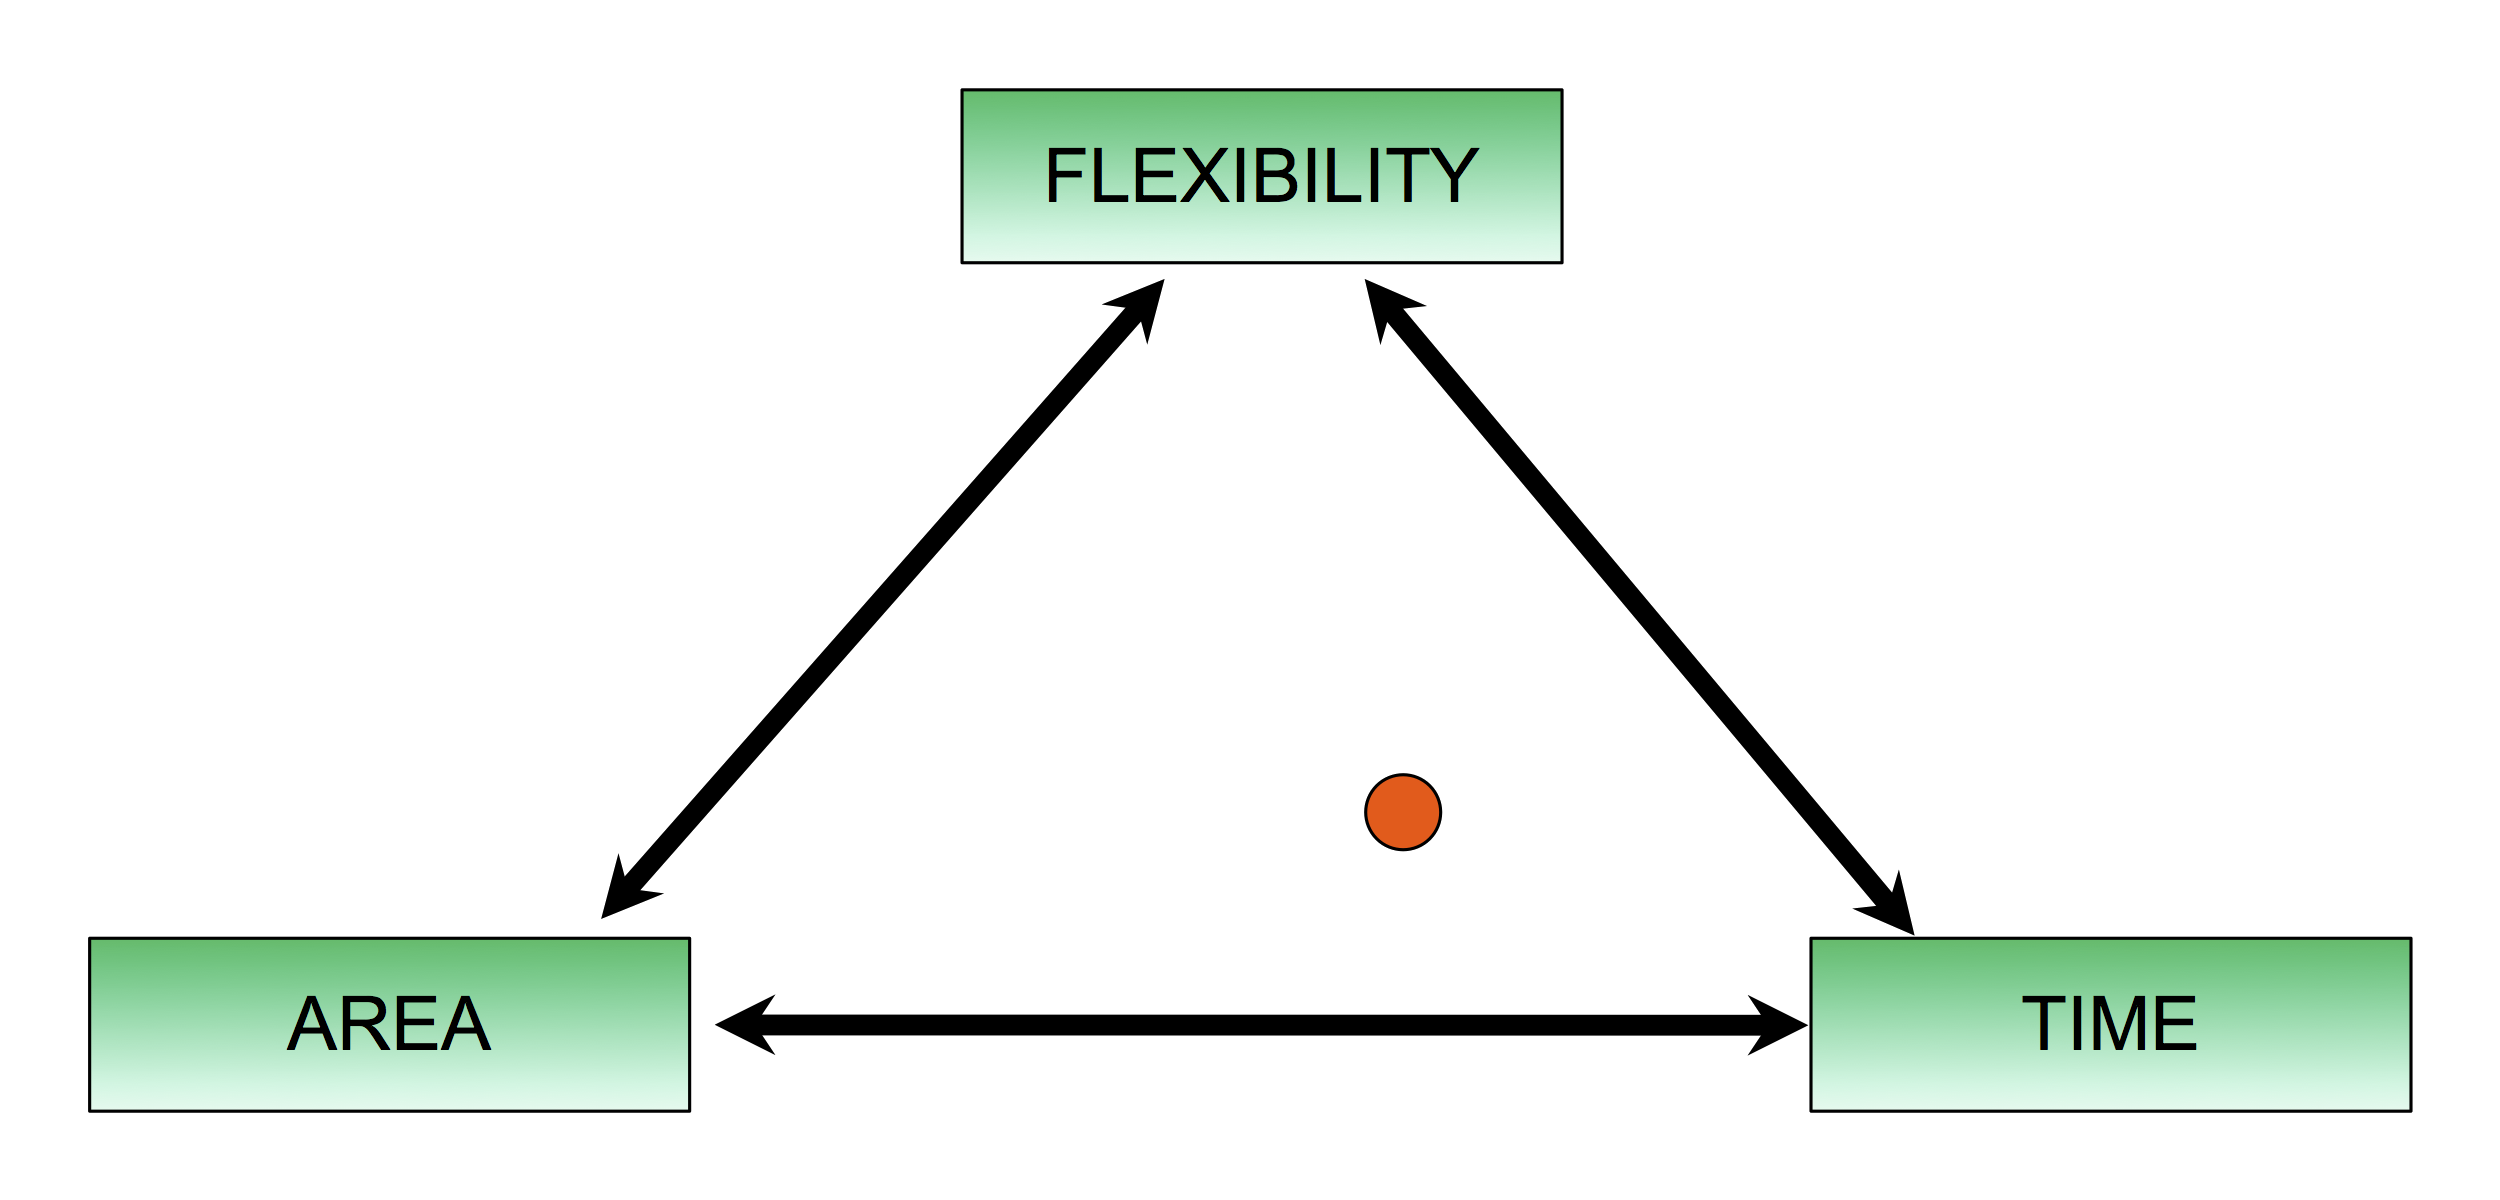
\includegraphics[width=0.5\linewidth]{situation_winter.png}}
	\caption{Situation---Winter}
	\label{fig:situation_winter}
\end{figure}

\section{Overall Architecture}
\label{sec:overall_architecture}

Because a complete hardwire implementation was not necessarily faster, when rebuilding the project I decided to rely more on the microprocessor for the exponentiation. Additionally, the coprocessor's size had to be reduced considerably while increasing its maximum frequency. I also wanted to achieve this while keeping the cycle count at least the same.\\

\begin{figure}[H]
	\center{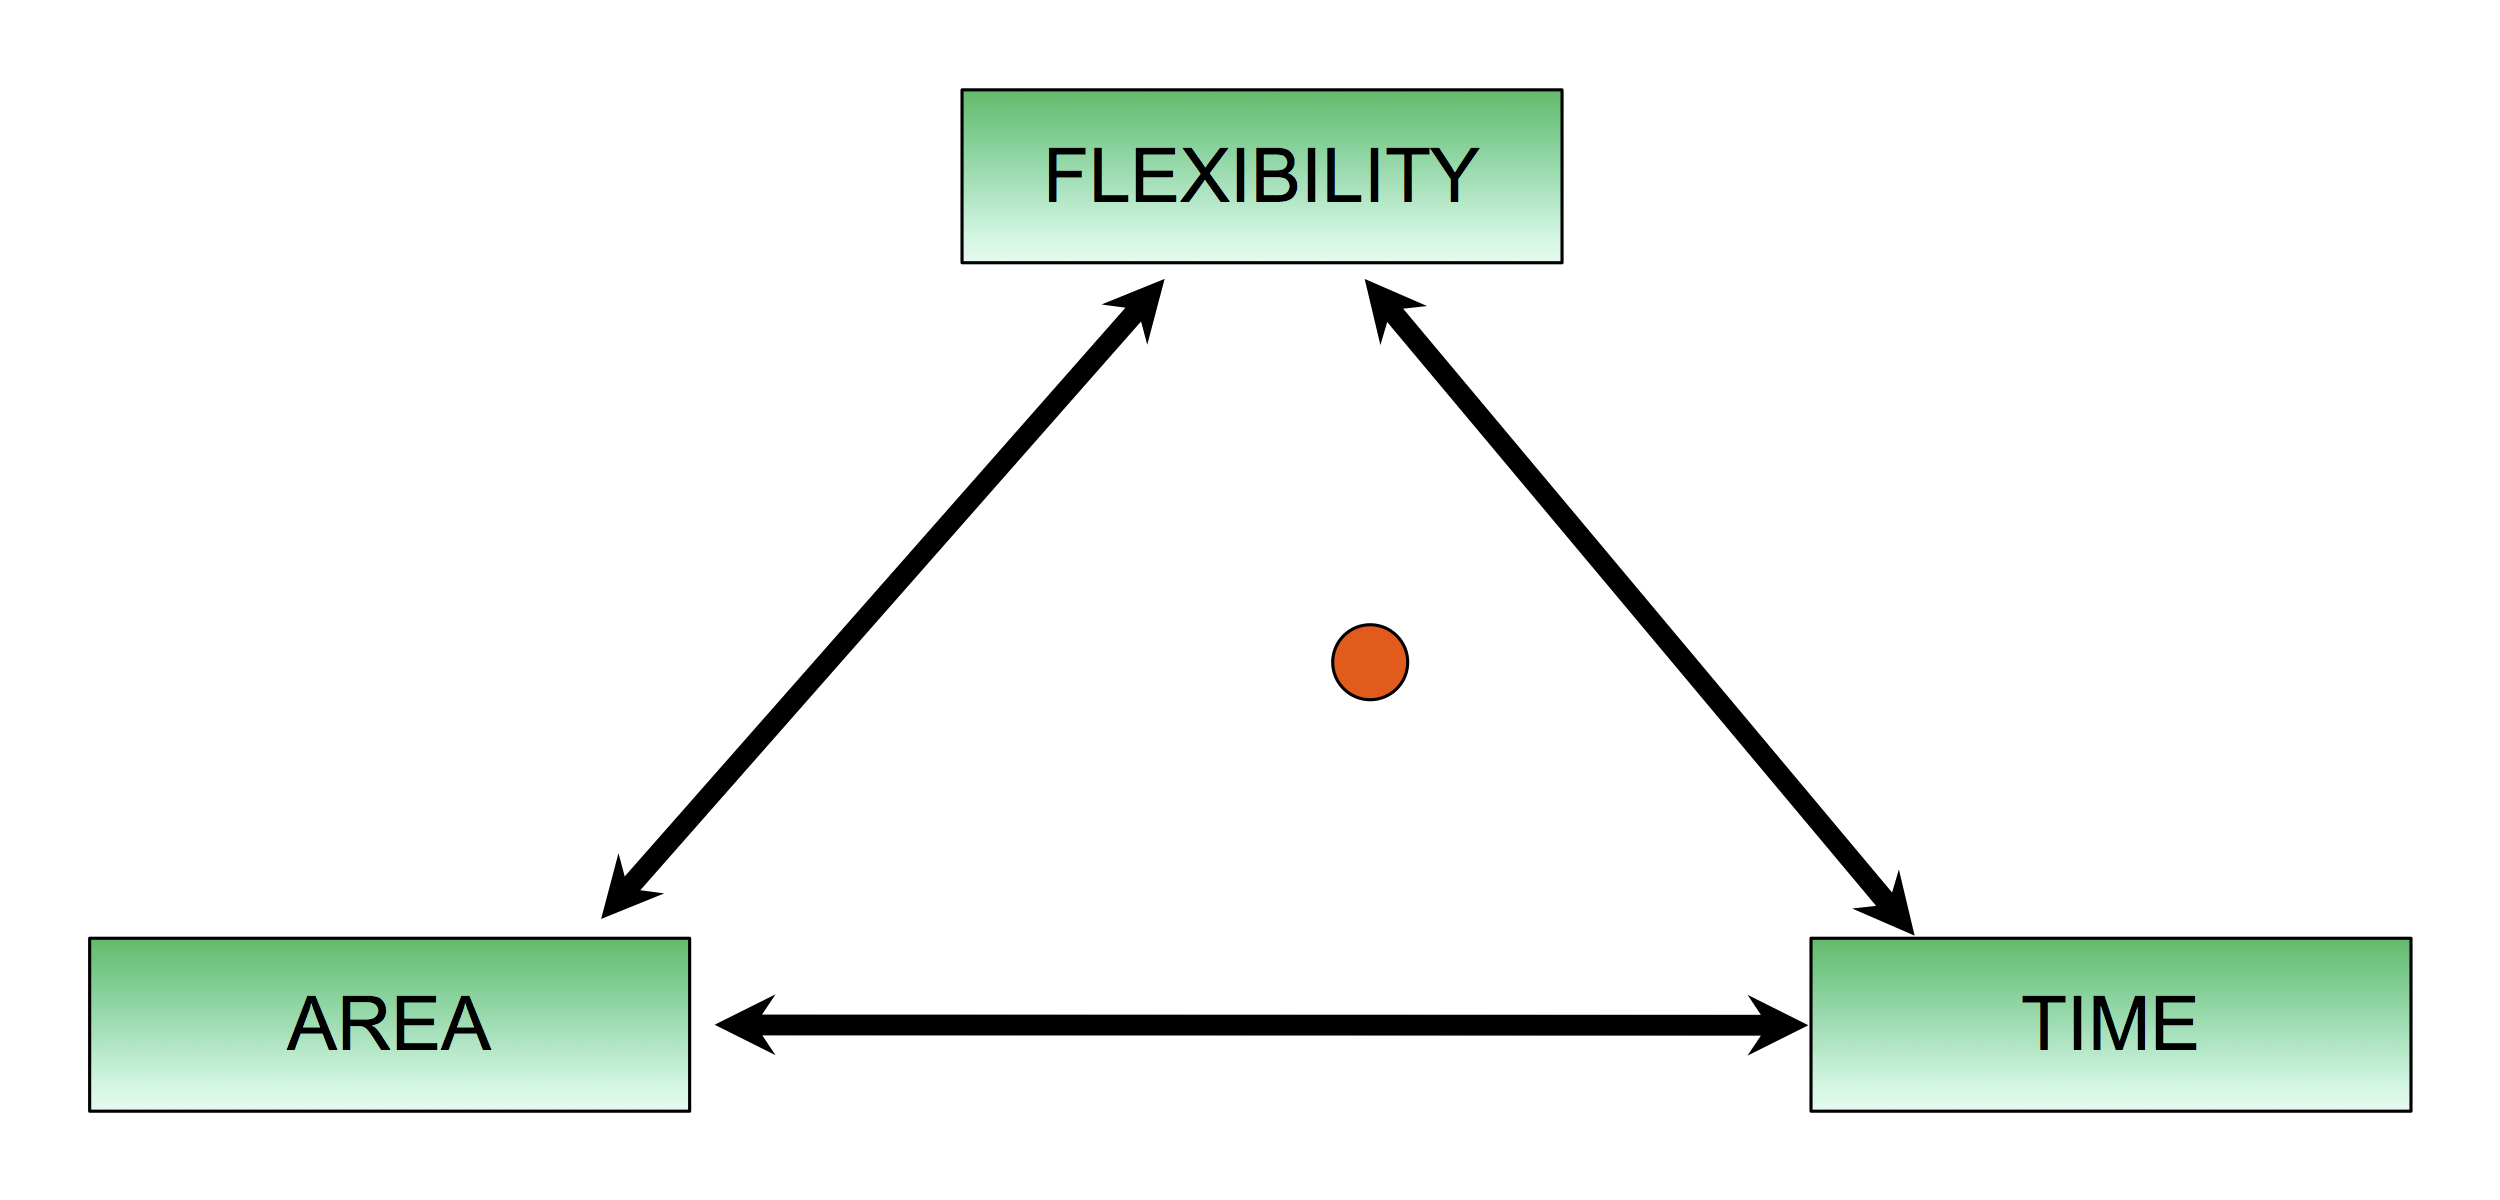
\includegraphics[width=0.5\linewidth]{situation.png}}
	\caption{Situation}
	\label{fig:situation_winter}
\end{figure}

Doing more in software resulted in greater flexibility during the development process. It made it easier to optimise  code and  future, more complex algorithmic optimisations possible (which may be supported by additional hardware features in the coprocessor). It also alloweded to reduce the size of the coprocessor considerably. An additional flexibility goal was easy integration into applications by providing a clear API and avoiding optimisations for specific parameters. The coprocessor should be as small as possible, but our primary goal is performance: if a considerable speed gain can be found by increasing the size, this will be implemented.\\

Starting from the existing decoder and Montgomery multiplier from the winter submissions, I built a hardware Montgomery multiplier that was fully memory-mapped. The different ports ($P1$-$P4$) were again used for the communication between the microprocessor and coprocessor. To reduce the overhead of copying data, instructions were introduced to write the multiplication parameters either from memory or from the result register.

\section{HW/SW Boundaries and Interface}
\label{sec:hwsw_boundaries_and_interface}

As mentioned before, the hardware only provides the Montgomery multiplier. The exponentiation algorithm itself is implemented in software on the microprocessor. Both the microprocessor and the coprocessor can access the same XRAM. We use this memory to exchange data between them.\\

The 8051 microprocessor has four one-byte ports we can use to communicate with the coprocessor. Instructions are put on port $P0$ and status signals are exchanged on port $P2$. $P3$ is a special port used only to send the terminate signal to the coprocessor.\\

The upper byte of a 2-byte address is sent to the coprocessor on port $P1$. From the specified address, the hardware reads a 128-byte parameter to the register specified by the register. Because the microprocessor is little-endian and the hardware big-endian, the bit order has to be reversed when reading and writing. As the full addresses are 2 bytes long, this means that we can only access half the memory right. If needed, this could be solved for example by introducing different read and write instructions depending on whether the first or last 128 bytes from the should be read or written.

\section{Performance Metrics}

\subsection{Clock Cycles}

The base release was built using the decoder and montgomery multiplier that was built in the winter, but with the exponentiation algorithm itself programmed in software. Because our hardware design had been very modular, it was fairly easy to take the parts I needed and build the initial version of the new coprocessor. As we can see from Table~\ref{tab:clock_cycles}, this resulted in a very slow implementation, taking more than half a billion cycles. The main reason for this was that I was still using the four shared memory locations for the multiplication factors, the modulus and the result. Because of this, data had to be copied to and from these locations by the microprocessor, which is very slow.\\

\begin{table}[H]
    \begin{center}	
        \begin{tabular}{l|r|r}
            & \textbf{Total} & \textbf{Change}\\\hline
            \textbf{Base} & 576456696 & \\
            \textbf{Memory} & 38191608 & -93.37\%\\
            \textbf{Full Memory} & 4412878 & -88.45\%\\
            \textbf{No Montgomery DP} & 4244100 & -3.82\%\\
            \textbf{Reduced Idling} & 2801376 & -33.99\%\\
            \textbf{Critical Path} & 2802636 & 0.04\%\\
            \textbf{Final} & 2732760 & -2.49\%
		\end{tabular}
	\end{center}
	\caption{Clock Cycles---Total}
	\label{tab:clock_cycles_total}
\end{table}

When analysing the algorithm, it become clear that the result of the previous multiplication is often used as either one or both of the multiplication factors. By creating additional instructions that specify whether the factors had to be read from the result register or from the memory, the required number of cycles was reduced by 93.37\%.\\

However, having to copy data back and forth between the four shared memory locations was a serious drawback. This design had made sense when the exponentiation had been fully implemented in hardwire, as we only had to copy the different parameters at the start and then retrieve the result after the hardware was done. However, for the exponentiation implemented in software parameters needed to be transferred a lot more often which resulted in a large amount of copying. This could be solved by allowing the hardware to read and write its data from any memory location. Therefore, instead of using a small number of hardcoded memory locations, the upper byte of the address is communicated to the coprocessor and it can read or write a 128 byte parameter from any location in the XRAM (see Paragraph~\ref{sec:hwsw_boundaries_and_interface}).\\

Next, I noticed that a lot of cycles were lost between the coprocessor finishing a montgomery multiplication and the microprocessor issuing the next instruction. The number of idle cycles was reduced by letting the coprocessor signal the microprocessor on $P2$ that the multiplication was done. By doing this, the next instruction is sent to the coprocessor sooner and less cycles are lost doing nothing.\\

\begin{table}[H]
    \begin{center}	
        \begin{tabular}{l|r|r}
            & \textbf{Encryption} & \textbf{Decryption}\\\hline
            \textbf{Base} & 4598424 & 571858272\\
            \textbf{Memory} & 605124 & 37586484\\
            \textbf{Full Memory} & 111540 & 4301338\\
            \textbf{No Montgomery DP} & 110652 & 4133448\\
            \textbf{Reduced Idling} & 96984 & 2704392\\
            \textbf{Critical Path} & 97044 & 2705592\\
            \textbf{Final} & 96192 & 2636568
		\end{tabular}
	\end{center}
	\caption{Clock Cycles---Encryption and Decryption}
	\label{tab:clock_cycles_encryption_and_decryption}
\end{table}

Finally, some small code optimisations were made. The function calls to \textit{montMultiply\_Single}, \textit{montMultiply\_Both} and \textit{MontMultiply\_Result} in \textit{montModExp} were manually inlined. The functions encapsulating the hardware calls were specified to be \textit{static inline} so that the compiler would inline them. The first iteration of the exponentiation could be extracted because $\text{Mont}(R\mod{m}, R\mod{m}) = R\mod{m}$.\\

Comparing the results from Table~\ref{tab:performance_metrics_winter} and Table~\ref{tab:clock_cycles_encryption_and_decryption} we can see that although the encryption is about 25000 in the new design, the decryption is almost 450000 cycles faster. To have at least the same cycle count was one of the goals for the new design (see Paragraph~\ref{sec:overall_architecture}).

\subsection{Time}

As we will see in Paragraph~\ref{sec:synthesis_results} the clock frequency was initially 11.524 \mega\hertz. This resulted in an execution time of 50.02 seconds to initialise the processor, encrypt the message and decrypt it. After optimisations, the final clock frequency is 25.076 \mega\hertz\ and the final execution time is reduced to 0.109 seconds. This is a lot less than the 0.273 seconds for the winter design.

\subsection{Area}

The initial design needed six large registers because the separate multiplication data path needed one register to store the shifted first factor and another for the result. By integrating this data path in the one of the decoder, these registers could be removed. Therefore the new implementation only needs four large registers where the old one needed 12.\\

\begin{table}[H]
	\begin{center}	
		\begin{tabular}{l|r}
			& \textbf{Registers} (Bit)\\\hline
        		\textbf{Base} & 6186\\
             \textbf{No Montgomery DP} & 4135\\
             \textbf{Critical Path} & 4136
		\end{tabular}
	\end{center}
	\caption{Registers}
	\label{tab:registers}
\end{table}

\section{Synthesis Results}
\label{sec:synthesis_results}

Synthesising the generated VHDL code was relatively straightforward in Xilinx. The only error encountered was that the process failed when the instruction register was compared to a hexadecimal numbers in the FSM. This was fixed by changing them to their decimal form.\\

From Table~\ref{tab:synthesis_results} we can see that the clock frequency of the base design was even slower than that of the winter design. After the integration of the multiplication data path, the clock frequency increased a bit to 13.141 \mega\hertz. However, analyses of the critical path revealed that we could do better. At the end of the Montgomery multiplication there is an overflow check which will add the modulus when needed.\\

As we can see from the following code fragment, where y\_sig is the second term that is passed to the adder data path, there is both a comparator and an adder in the critical path. This is the main reason that the frequency of our coprocessor is so low.

\begin{lstlisting}
sfg mont_overflow_check {
    ...
    y_sig = r_reg >= m_reg ? m_reg : 0;
    ...
}
\end{lstlisting}

We can solve this problem by moving the comparison and addition to separate cycles. This was done by introducing one additional register to hold the result of the comparison and introducing two additional states to our FSM. This will introduce some extra cycles to the execution as can be verified from the numbers in Table~\ref{tab:clock_cycles_total}). However, this increased cycle count is very small relative to the total number of cycles. And more importantly, the frequency of the coprocessor is almost doubled to 25.076.\\

\begin{table}[H]
	\begin{center}	
		\begin{tabular}{l|r|r|r|r}
			& \textbf{Slices} & \textbf{Slice FFs} & \textbf{4 Input LUTs} & \textbf{Frequency} (\mega\hertz)\\\hline
        		\textbf{Base} & 13891 (54\%) & 6219 (12\%) & 26485 (52\%) & 11.524\\
             \textbf{No Montgomery DP} & 8304 (32\%) & 4138 (8\%) & 15774 (31\%) & 13.141\\
             \textbf{Critical Path} & 8116 (32\%) & 4145 (8\%) & 15336 (30\%) & 25.076
		\end{tabular}
	\end{center}
	\caption{Synthesis Results}
	\label{tab:synthesis_results}
\end{table}

Aside from the clock frequency, we can also clearly see the impact of the reduced number of registers here. Where the old design used 63\% of the available slices and 24\% of the available slice flip flops (see Table~\ref{tab:synthesis_results_winter}), the new one only uses 32\% and 8\% respectively.

\section{Test Strategy}

To debug the C code syntactically, we can rely on the compiler. However, the GEZEL's cosimulation platform does not have any dedicated tools to debug the design. Therefore, testing and profiling is done ad-hoc by displaying and comparing (intermediate) results. The debugging was mostly done against the encryption process because it has fewer loop iterations. The results used for the comparison were obtained by creating a Maple worksheet with all the steps of the Montgomery exponentiation.\\


To make this process a bit easier, two instructions were added: one to report the nummer of cycles and the other to display the contents of the result register. By sending these instructions to the coprocessor, we can view both at any given moment. Aside from our dedicated instructions, the \textit{\$display} statement in GEZEL also came in handy to display the contents of registers other than the result register. By issuing the display cycles instruction around blocks of code, the design could be profiled. It also allowed me to verify the effect of a given optimisation.

\section{Further Optimisations}

The current implementation is relatively fast, but we still could do better. Especially the decryption process takes a long time and speeding it up would be good. In a smartcard RSA is usually used to create a digital signature. A message is signed with the private key (our decryption process) and that signature is verified with the public key. So it makes sense to spend a bit more time optimising the decryption, as it will be used often.\\

From the course \textit{Cryptography and Network Security} and from having implemented RSA for the \textit{P\&D Multimedia} I know that by applying the Chinese Remainder Theorem to its modular exponentiation, the decryption can be sped up considerably. The modulus $m$ is actually the product of two primes $p$ and $q$. The CRT takes advantage of this and calculates two exponentiations with shorter exponents (see Handbook of Applied Cryptography, Chapter 14, Algorithm 14.71). Their results are then recombined to form $x^e\mod{m}$.

\end{document}